% 题面依据2011-02-01公开旧讲义，PDF78--81、96--97。
% 未见公开官方解答；本文件解答为编者独立编写，印刷问题显式登记。
\originalsection{Homework 10：箭图与 McKay 图}
本次作业的原题是旧讲义的5.1--5.5，其中5.5的末两问在原PDF第81页。题面译自公开旧讲义，以下解答由AI辅助独立编写，并非MIT官方答案。为解答这些题，本节补充箭图、Dynkin图和根格的必要知识；这些局部补充不表示本书已覆盖旧讲义的箭图、李代数或一般有限维代数全部专题。以下默认箭图表示有限维，底域代数闭；涉及特征标和有限旋转群时取底域为 $\C$。

\begin{exercise}\label{hw:5.1}
\textbf{MIT 18.712（2010）Homework 10 原题5.1；旧PDF第78页。}
设 $k$ 是域，$k(y_1,\ldots,y_m)$ 是 $m$ 个变量上的有理函数域。若有单射的 $k$-代数同态
\[
 f:k[x_1,\ldots,x_n]\longrightarrow k(y_1,\ldots,y_m),
\]
证明 $m\ge n$。原题提示：比较 $x_i$ 中次数为 $N$ 的多项式空间及其像随 $N\to\infty$ 的维数增长。再推得，若有 $k$-域嵌入 $k(x_1,\ldots,x_n)\to k(y_1,\ldots,y_m)$，仍有 $m\ge n$。
\end{exercise}
\begin{solution}
为得到足够强的增长率，使用\textbf{总次数至多} $N$ 的空间 $W_N$，而非只取齐次次数恰为 $N$ 的空间。其单项式基给出
\[
 \dim_k W_N=\binom{N+n}{n}.
\]
把所有 $f(x_i)$ 写成共同分母的形式 $p_i/q$，其中 $p_i,q\in k[y_1,\ldots,y_m]$，$q\ne0$。取 $D\ge1$，使这些多项式的总次数都不超过 $D$。若 $x^\alpha$ 的次数 $|\alpha|\le N$，则
\[
 q^N f(x^\alpha)=q^{N-|\alpha|}\prod_i p_i^{\alpha_i}
\]
是次数至多 $DN$ 的多项式。因此，$f$ 的单射性和乘以 $q^N$ 的单射性共同给出
\[
 \binom{N+n}{n}\le\binom{DN+m}{m}\qquad(N\ge0).
\]
左侧关于 $N$ 的次数为 $n$，右侧为 $m$，且最高次系数都为正。若 $n>m$，当 $N$ 足够大时不等式不可能成立，故 $n\le m$。域嵌入限制到多项式子代数仍然单射，第二个结论随即成立。
\end{solution}

\begin{exercise}\label{hw:5.2}
\textbf{MIT 18.712（2010）Homework 10 原题5.2；旧PDF第78页。}
设 $k$ 代数闭，$G=\GL_n(k)$，$V$ 是 $G$ 的多项式表示。证明：若 $G$ 在 $V$ 上只有有限个轨道，则 $\dim V\le n^2$。
\begin{enumerate}[label=(\alph*)]
\item 取 $V$ 的线性坐标 $x_1,\ldots,x_N$。称子集 $X\subset V$ 为Zariski稠密，如果在 $X$ 上为零的多项式只能是零多项式。证明有限个轨道中至少有一个Zariski稠密轨道。
\item 据此构造域嵌入 $k(x_1,\ldots,x_N)\to k(g_{pq})$，再用原题5.1。
\item 推广到 $G=\GL_{n_1}(k)\times\cdots\times\GL_{n_s}(k)$。
\end{enumerate}
\end{exercise}
\begin{solution}
\textbf{(a)} 若所有轨道 $O_1,\ldots,O_t$ 都不稠密，可为每个轨道取非零多项式 $F_j$，使 $F_j|_{O_j}=0$。则非零多项式 $\prod_jF_j$ 在整个 $V=k^N$ 上为零。代数闭域是无限域，而无限域上在所有点取零值的多项式必为零：对变量数归纳，把它当作最后一个变量的一元多项式，并用一元非零多项式的根数有限。这一矛盾证明了结论。

\textbf{(b)} 取稠密轨道中的点 $v$。轨道映射 $g\mapsto gv$ 把坐标函数 $x_i$ 拉回为矩阵坐标 $g_{pq}$ 的多项式，因而定义同态
\[
 k[x_1,\ldots,x_N]\longrightarrow k(g_{pq}),\qquad F\longmapsto[g\mapsto F(gv)].
\]
若像为零，$F$ 在稠密轨道上消失，故 $F=0$；同态单射，并能唯一延拓到分式域。目标有 $n^2$ 个变量，原题5.1给出 $N\le n^2$。

\textbf{(c)} 相同证明给出
\[
 \boxed{\dim V\le\sum_{j=1}^s n_j^2.}
\]
下一题需要稍宽的版本：作用矩阵的系数可以是矩阵坐标及行列式的逆所组成的有理函数。此时轨道映射的拉回仍落在同一有理函数域，以上单射和变量数论证完全保留。因此结论也适用于这种有理表示，而不必强求所有系数都是多项式。
\end{solution}

\begin{exercise}\label{hw:5.3}
\textbf{MIT 18.712（2010）Homework 10 原题5.3；旧PDF第78--80页。}
设 $\Gamma$ 是有限连通无自环图，允许重边，顶点为 $1,\ldots,N$。令 $r_{ij}$ 为 $i,j$ 间的边数，$R_\Gamma=(r_{ij})$，$A_\Gamma=2I-R_\Gamma$。若 $A_\Gamma$ 定义的实二次型正定，称 $\Gamma$ 为Dynkin图。证明这类图恰为 $A_n$（$n\ge1$）、$D_n$（$n\ge4$）、$E_6,E_7,E_8$。

为准确说明原题的图形，$A_n$ 是 $n$ 个顶点的链；$D_n$ 是从一个三价顶点伸出长度为 $n-3,1,1$ 的三条臂；$E_6,E_7,E_8$ 的三臂长度分别为 $(2,2,1),(3,2,1),(4,2,1)$。这里臂长是边数，中心不重复计入。下图逐一重画旧讲义第78--79页的有限型图：
\begin{center}
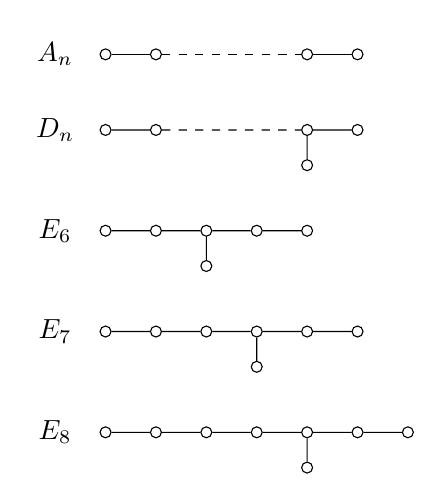
\begin{tikzpicture}[scale=.64,every node/.style={circle,draw,fill=white,inner sep=1.4pt}]
\node[draw=none] at (-1,0) {$A_n$};
\foreach \i in {0,1,4,5}{\node (a\i) at (\i,0) {};}
\draw (a0)--(a1);\draw[dashed] (a1)--(a4);\draw (a4)--(a5);
\node[draw=none] at (-1,-1.5) {$D_n$};
\foreach \i in {0,1,4,5}{\node (d\i) at (\i,-1.5) {};}
\node (db) at (4,-2.2) {};\draw (d0)--(d1);\draw[dashed] (d1)--(d4);\draw (d4)--(d5);\draw (d4)--(db);
\node[draw=none] at (-1,-3.5) {$E_6$};
\foreach \i in {0,...,4}{\node (s\i) at (\i,-3.5) {};}
\node (sb) at (2,-4.2) {};\foreach \i [evaluate=\i as \j using int(\i+1)] in {0,...,3}{\draw (s\i)--(s\j);}\draw (s2)--(sb);
\node[draw=none] at (-1,-5.5) {$E_7$};
\foreach \i in {0,...,5}{\node (t\i) at (\i,-5.5) {};}
\node (tb) at (3,-6.2) {};\foreach \i [evaluate=\i as \j using int(\i+1)] in {0,...,4}{\draw (t\i)--(t\j);}\draw (t3)--(tb);
\node[draw=none] at (-1,-7.5) {$E_8$};
\foreach \i in {0,...,6}{\node (u\i) at (\i,-7.5) {};}
\node (ub) at (4,-8.2) {};\foreach \i [evaluate=\i as \j using int(\i+1)] in {0,...,5}{\draw (u\i)--(u\j);}\draw (u4)--(ub);
\end{tikzpicture}
\end{center}
\begin{enumerate}[label=(\alph*)]
\item 用按行展开建立递推，计算 $A_N,D_N$ 的Cartan矩阵行列式，并用Sylvester判据证明正定。
\item 计算 $E_6,E_7,E_8$ 的行列式并证明正定。
\item 证明Dynkin图没有圈。原题提示：圈图的Cartan矩阵各行之和为零。
\item 证明其顶点度数至多三，且三价顶点至多一个。原题给出的禁图为四臂星形，以及两个三价顶点由一条链连接、各自另接两个叶子的图。
\item 证明三臂长度分别为 $(2,2,2),(3,3,1),(5,2,1)$ 的图的Cartan矩阵行列式为零。这是原题第79--80页的三个带数字禁图。
\item 由以上结果完成有限型分类。
\item 分类仿射Dynkin图。原题把它定义为Cartan矩阵半正定的连通无自环图，并要求它们恰为前面的禁图。
\end{enumerate}
\end{exercise}
\begin{remark}
原题(g)的定义少了“非正定”这一条件：正定矩阵本来也是半正定矩阵，照字面会把有限型全部包含进去。以下将“仿射”按半正定而非正定解释；若严格沿用原题字面，则答案应是有限型与仿射型的并集。允许重边时还须补入两个顶点之间的双边图 $\widetilde A_1$，它是长度二的圈；旧图中没有单独画出这个边界情形。
\end{remark}
\begin{solution}
先记两个可重复使用的计算。若树 $T$ 中的叶子 $v$ 邻接 $u$，沿叶子所在行、列展开，有
\[
 \Delta(T)=2\Delta(T-v)-\Delta(T-\{u,v\}),\qquad
 \Delta(T)=\det A_T.
\]
删掉顶点后若图不连通，行列式就是各连通分支行列式的乘积；空图的行列式取一。

\textbf{(a)} 令 $d_n=\Delta(A_n)$，则 $d_0=1,d_1=2$，且 $d_n=2d_{n-1}-d_{n-2}$，归纳得到 $d_n=n+1$。链按顺序编号时，各顺序主子式为 $2,3,\ldots,n+1$，故由Sylvester判据正定。对 $D_n$，删去其中一个短臂叶子，剩下 $A_{n-1}$；再删去中心，剩下 $A_{n-3}$ 与一个孤立点。因此
\[
 \Delta(D_n)=2n-2(n-2)=4.
\]
先编号长臂、中心和一个短臂，最后编号另一个短臂，则前 $n-1$ 个顺序主子式来自链，最后一个为四，全部为正。

\textbf{(b)} 将三臂图记为 $T(a,b,c)$。一条长度为 $a$ 的臂对应链矩阵 $A_{A_a}$，其靠中心端的逆矩阵对角元为
\[
 (A_{A_a}^{-1})_{11}=\frac{\Delta(A_{a-1})}{\Delta(A_a)}=\frac a{a+1}.
\]
先消去三条臂，中心的Schur补为
\[
 2-\frac a{a+1}-\frac b{b+1}-\frac c{c+1}
 =\frac1{a+1}+\frac1{b+1}+\frac1{c+1}-1.
\]
于是
\[
 \Delta(T(a,b,c))=(a+1)(b+1)(c+1)
 \left(\frac1{a+1}+\frac1{b+1}+\frac1{c+1}-1\right).
\]
代入 $(2,2,1),(3,2,1),(4,2,1)$，依次得到 $3,2,1$。先给水平链编号，最后给短臂叶子编号，前面的主子式都为链的正行列式，最后一个也为正，故三图正定。

\textbf{(c)--(e)} 若 $A_\Gamma$ 正定，则任何子图也必须正定。这里对子图允许删边：若子图非正定，先取非零向量 $x$ 使其二次型不正，再改为 $d=|x|$；由于非对角项非正，二次型不会增加。将 $d$ 在其余顶点上延伸为零，增加边只会再减去非负项。因此找到这样的子图就足以排除正定性。

圈图取所有 $d_i=1$，则 $A_\Gamma d=0$。若有重边，两个端点上的矩阵为 $\bigl(\begin{smallmatrix}2&-r\\-r&2\end{smallmatrix}\bigr)$，当 $r\ge2$ 时在 $(1,1)$ 上不正，所以正定图必是没有重边的树。

四臂星形取中心权二、叶子权一，满足每个顶点的“两倍自身权等于相邻权之和”。有两个三价顶点时，取连接它们的整条链上的权为二，两端另外四个叶子的权为一，同样满足 $Ad=0$。若原树有更多分叉，取两分叉间最短路径，并截取两端各两条支边，仍得到该禁图。因此最大度数不超过三，三价顶点至多一个。

三个例外禁图的非零核向量如下。图的数字和连接关系按旧讲义第79--80页重画，数字都是顶点权，而不是顶点编号：
\begin{center}
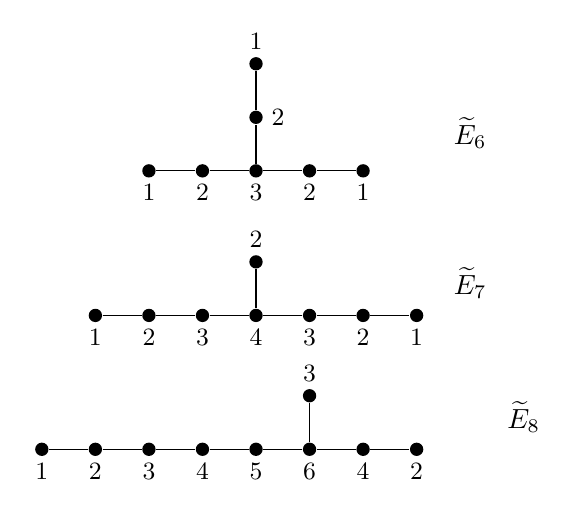
\begin{tikzpicture}[scale=.68,every node/.style={circle,fill=black,inner sep=1.7pt},every label/.style={fill=none,draw=none,font=\small,inner sep=1pt}]
\node[label=below:1] (e60) at (-2,0) {};\node[label=below:2] (e61) at (-1,0) {};\node[label=below:3] (e62) at (0,0) {};\node[label=below:2] (e63) at (1,0) {};\node[label=below:1] (e64) at (2,0) {};\node[label=right:2] (e65) at (0,1) {};\node[label=above:1] (e66) at (0,2) {};
\draw (e60)--(e61)--(e62)--(e63)--(e64);\draw (e62)--(e65)--(e66);
\node[fill=none] at (4,0.7) {$\widetilde E_6$};
\foreach \i/\w in {0/1,1/2,2/3,3/4,4/3,5/2,6/1}{\node[label=below:\w] (e7\i) at (\i-3,-2.7) {};}
\foreach \i [evaluate=\i as \j using int(\i+1)] in {0,...,5}{\draw (e7\i)--(e7\j);}
\node[label=above:2] (e77) at (0,-1.7) {};\draw (e73)--(e77);\node[fill=none] at (4,-2.1) {$\widetilde E_7$};
\foreach \i/\w in {0/1,1/2,2/3,3/4,4/5,5/6,6/4,7/2}{\node[label=below:\w] (e8\i) at (\i-4,-5.2) {};}
\foreach \i [evaluate=\i as \j using int(\i+1)] in {0,...,6}{\draw (e8\i)--(e8\j);}
\node[label=above:3] (e88) at (1,-4.2) {};\draw (e85)--(e88);\node[fill=none] at (5,-4.6) {$\widetilde E_8$};
\end{tikzpicture}
\end{center}
逐点检查 $2d_i=\sum_{j\sim i}d_j$ 即得 $Ad=0$，故三者行列式为零。前两类禁图也可带权画成
\begin{center}
\begin{tikzpicture}[scale=.68,every node/.style={circle,fill=black,inner sep=1.7pt},every label/.style={fill=none,draw=none,font=\small,inner sep=1pt}]
\foreach \i in {0,...,4}{\node[label={\i*72:1}] (c\i) at (\i*72:1) {};}
\foreach \i/\j in {0/1,1/2,2/3,3/4,4/0}{\draw (c\i)--(c\j);}
\node[fill=none] at (0,-1.8) {圈：全为一};
\node[label=below:2] (l) at (3.2,0) {};\node[label=below:2] (r) at (6,0) {};
\node[label=above:1] (ll) at (2.3,.8) {};\node[label=below:1] (ld) at (2.3,-.8) {};
\node[label=above:1] (rr) at (6.9,.8) {};\node[label=below:1] (rd) at (6.9,-.8) {};
\draw (ll)--(l)--(ld);\draw[dashed] (l)--(r);\draw (rr)--(r)--(rd);
\node[fill=none] at (4.7,-1.8) {$\widetilde D_n$：中间链全为二};
\end{tikzpicture}
\end{center}
右图的两个分叉点重合时成为 $\widetilde D_4$：中心权二，四个叶子权一；圈的两个顶点由双边相连时成为 $\widetilde A_1$。

\textbf{(f)} 没有三价顶点的树是 $A_n$。有唯一三价顶点时是 $T(a,b,c)$，设 $1\le a\le b\le c$。正定等价于
\[
 \frac1{a+1}+\frac1{b+1}+\frac1{c+1}>1.
\]
若 $a\ge2$，左侧至多一，故 $a=1$。若 $b=1$，任意 $c\ge1$ 都成立，给出 $D_{c+3}$；若 $b=2$，则必须 $c=2,3,4$，给出 $E_6,E_7,E_8$；若 $b\ge3$，左侧又至多一。分类完成。

\textbf{(g)} 对上述每个禁图，已写出正核向量 $d$。把重边按条计数，有恒等式
\[
 x^{\mathsf T}Ax=
 \sum_{\{i,j\}\text{为边}}d_i d_j
 \left(\frac{x_i}{d_i}-\frac{x_j}{d_j}\right)^2.
\]
展开后，$x_i^2$ 的系数为 $\sum_{j\sim i}d_j/d_i=2$，交叉项为每条边的 $-2x_ix_j$，故恒等式成立。它证明半正定；连通性又使核恰为 $\R d$。

反之，设连通图的 $A$ 半正定且奇异。取非零核向量 $x$，则
$|x|^{\mathsf T}A|x|\le x^{\mathsf T}Ax=0$，故 $|x|$ 也在核中。若其某坐标为零，核方程迫使所有邻点坐标为零，连通性将迫使全部为零。因此有严格正的核向量。一个具有正核向量的禁图不能真包含在更大的连通半正定图中：增加其内部边立即使该向量的二次型为负；增加相邻顶点时，把旧向量延伸为零虽仍有零二次型，却不再满足核方程，而半正定矩阵的零二次型向量必须在核中，矛盾。

如果该图没有任何禁图，前面的分类已经证明它属于正定的有限型，与奇异性矛盾；所以它恰是一个禁图。由此全部仿射型为圈 $\widetilde A_{r-1}$（$r\ge3$）、双边 $\widetilde A_1$、$\widetilde D_n$（$n\ge4$）以及 $\widetilde E_6,\widetilde E_7,\widetilde E_8$。
\end{solution}

\begin{exercise}\label{hw:5.4}
\textbf{MIT 18.712（2010）Homework 10 原题5.4；旧PDF第80页。}
设 $Q$ 的顶点集为 $D$。若 $Q$ 的不可分解有限维表示只有有限个同构类，称 $Q$ 为有限型。令 $b_{ij}$ 是从 $i$ 到 $j$ 的箭头数。Gabriel定理说：连通箭图是有限型，当且仅当忘掉箭头方向后得到Dynkin图。本题只证明必要性。
\begin{enumerate}[label=(\alph*)]
\item 证明有限型迫使相应二次型在 $x_i\in\mathbb Q$、$x_i\ge0$ 且不全为零的向量上为正。原题印刷的二次型是
\[
 q_{\text{印}}(x)=\sum_i x_i^2-\frac12\sum_{i,j}b_{ij}x_ix_j.
\]
提示先取非负整数 $n_i$，考虑所有维数为 $n_i$ 的表示组成的空间 $W$，使 $\prod_i\GL_{n_i}(k)$ 在 $W\oplus k$ 上具有有限轨道，利用原题5.2，再推广到任意整数和有理数。
\item 推出二次型正定。原题提示利用 $\mathbb Q$ 在 $\R$ 中稠密。
\item 排除自环，再利用原题5.3得到Gabriel定理的必要性。
\end{enumerate}
\end{exercise}
\begin{remark}
按原题给定的\textbf{有向}箭头数 $b_{ij}$，用于Gabriel定理的二次型应为
\[
 q_Q(x)=\sum_i x_i^2-\sum_{i,j}b_{ij}x_ix_j.
\]
原印刷式的 $1/2$ 是多余的。若改用无向对称邻接矩阵 $R$，才可写成 $q_Q(x)=\sum_i x_i^2-\tfrac12\sum_{i,j}R_{ij}x_ix_j$（此处无自环）。例如Kronecker箭图的 $b_{12}=2$，原印刷式成为 $x_1^2+x_2^2-x_1x_2$，正定但图并非有限型，不能据此证明(c)。以下使用修正后的 $q_Q$，并完整证明原题意图中的必要性。
\end{remark}
\begin{solution}
箭图的一个表示给每个顶点 $i$ 一个向量空间 $V_i$，给每条箭头 $i\to j$ 一个线性映射 $V_i\to V_j$；同构是在各顶点换基，并与所有箭头映射相容。固定非零维数向量 $n=(n_i)$，令
\[
 W=\bigoplus_{a:i\to j}\Hom_k(k^{n_i},k^{n_j}),\qquad
 H=\prod_{i:n_i>0}\GL_{n_i}(k).
\]
于是 $\dim W=\sum_{i,j}b_{ij}n_i n_j$，$\dim H$ 在本题的变量计数意义下是 $\sum_i n_i^2$。$H$ 以 $T_a\mapsto g_jT_ag_i^{-1}$ 作用，轨道恰是这些表示的同构类。

任一有限维表示可通过反复分解为较小维数的非零直和项，写成不可分解表示的直和。若不可分解同构类只有有限个，则固定总维数时，各类的重数有统一有限上界，因此只产生有限个同构类，$W$ 上只有有限轨道。

为了获得严格不等式，而非仅有非负性，选一个 $n_j>0$，使 $H$ 还在额外的一维空间上按 $z\mapsto(\det g_j)z$ 作用。每个 $W$ 轨道的稳定子都含有共同标量 $g_i=tI_{n_i}$；它在额外坐标上乘以 $t^{n_j}$。代数闭性保证非零数都有 $n_j$ 次根，所以该稳定子在额外坐标的非零值上作用传递。每个旧轨道恰贡献 $z=0$ 和 $z\ne0$ 两类轨道。因此 $W\oplus k$ 仍只有有限轨道。用原题5.2的有理作用版本，得到
\[
 \sum_{i,j}b_{ij}n_i n_j+1\le\sum_i n_i^2,
 \qquad\text{即 }q_Q(n)\ge1.
\]
若 $n$ 是任意非零整数向量，由箭头数非负可知
\[
 q_Q(n)\ge q_Q(|n|)>0.
\]
给有理向量乘以公共分母，再用二次齐次性，证明(a)。

\textbf{(b)} 连续性和有理点稠密首先只证明 $q_Q$ 半正定，\textbf{不能直接证明正定}。若它奇异，其矩阵有有理系数，所以高斯消元给出非零的有理核向量，与(a)矛盾。因此它确实正定。这一步补足了原提示中未写出的关键论证。

\textbf{(c)} 若顶点 $i$ 上有自环，令 $x_i=1$、其余为零，则 $q_Q(x)=1-b_{ii}\le0$，与正定性矛盾。无自环时，忘掉方向后的邻接矩阵满足
\[
 q_Q(x)=\frac12x^{\mathsf T}(2I-R)x.
\]
原题5.3的分类于是表明底图是Dynkin图。本题只得到Gabriel定理的“有限型必为Dynkin型”方向；反方向并未由这段维数论证证明。
\end{solution}

\begin{exercise}\label{hw:5.5}
\textbf{MIT 18.712（2010）Homework 10 原题5.5；旧PDF第80--81页。}
设 $G\ne\{1\}$ 是 $\mathrm{SU}(2)$ 的有限子群，$V$ 是由该嵌入得到的二维表示，$V_i$（$i\in I$）是全部不可约表示。令 $r_{ij}$ 为 $V_i$ 在 $V\otimes V_j$ 中的重数。
\begin{enumerate}[label=(\alph*)]
\item 证明 $r_{ij}=r_{ji}$。
\item McKay图 $M(G)$ 以 $i\in I$ 为顶点，并在 $i,j$ 之间连 $r_{ij}$ 条边。证明该图连通。原题提示利用原题3.26。
\item 证明它是原题5.3中的仿射Dynkin图。先证 $A=(2\delta_{ij}-r_{ij})$ 半正定而非正定，再证没有自环。原题提示：令 $F=\sum_i x_i\chi_{V_i}$，计算 $\langle(2-\chi_V)F,F\rangle$；非循环的有限 $\mathrm{SU}(2)$ 子群包含 $-I$。
\item 原题3.24中的各有限子群对应哪一种图？
\item 利用McKay图求这些群的全部不可约表示维数，证明它们就是原图中的顶点数字，并与原题3.24所得 $\mathrm{SO}(3)$ 子群比较。
\end{enumerate}
\end{exercise}
\begin{solution}
\textbf{(a)} $V$ 上的交替形式 $\omega(u,v)=\det(u,v)$ 在 $G$ 下不变且非退化，给出 $V\cong V^*$。由张量积与对偶的自然同态关系，
\[
 \Hom_G(V_i,V\otimes V_j)\cong\Hom_G(V\otimes V_i,V_j).
\]
Maschke定理使两边维数分别为 $r_{ij},r_{ji}$，故相等。也可用实值特征标 $\chi_V$ 和特征标内积验证这一等式。

\textbf{(b)} 嵌入保证 $V$ 忠实。原题3.26说明每个不可约表示出现在某个 $V^{\otimes n}$ 中。此处还可直接补一个特征标证明：$g\in\mathrm{SU}(2)$ 的特征值为 $e^{\mathrm i\theta},e^{-\mathrm i\theta}$，所以 $\chi_V(g)=2\cos\theta$，且 $\chi_V(g)=2$ 当且仅当 $g=1$。设不可约特征标 $\psi$ 与所有 $\chi_V^n$ 正交。按 $\chi_V$ 的有限个不同取值 $a$ 分组，得到对所有 $n\ge0$ 的等式
\[
 \sum_a a^n\sum_{g:\chi_V(g)=a}\overline{\psi(g)}=0.
\]
取 $n=0,\ldots,t-1$，Vandermonde矩阵可逆，各内层和都为零；但 $a=2$ 的内层和为 $\psi(1)=\dim\psi>0$，矛盾。于是每个不可约表示都能从平凡表示出发，沿连续张量乘以 $V$ 的分解到达，正好给出McKay图中的一条路，故图连通。

\textbf{(c)} 在不可约特征标正交基下，乘以 $\chi_V$ 的矩阵就是 $R=(r_{ij})$。对实向量 $x$ 和 $F=\sum_i x_i\chi_{V_i}$，
\[
 x^{\mathsf T}Ax=\langle(2-\chi_V)F,F\rangle
 =\frac1{|G|}\sum_{g\in G}(2-\chi_V(g))|F(g)|^2\ge0.
\]
取 $d_i=\dim V_i$，由 $\dim(V\otimes V_j)=2d_j$ 得到 $Rd=2d$，所以 $Ad=0$，不是正定矩阵。上式还说明，等号只可能出现在 $F$ 支持于单位元时；这样的类函数空间是一维的。因此 $\ker A$ 一维，正核向量 $d$ 将唯一确定全部维数，差一个共同倍数。

还须排除自环。如果 $G$ 非循环，由原题3.24的旋转群分类及 $\mathrm{SU}(2)\to\mathrm{SO}(3)$ 的核为 $\{I,-I\}$，它必包含 $-I$。具体说，如果不包含 $-I$，它没有二阶元素，因而阶数为奇数；其像是奇数阶旋转群，分类说明该像循环，而原群嵌入同一旋转轴的逆像（一个圆群），也只能是循环群。中央元 $-I$ 在每个不可约 $V_i$ 上按某个 $\varepsilon_i=\pm1$ 作用，在 $V$ 上按 $-1$ 作用。因此 $V\otimes V_i$ 的中央符号为 $-\varepsilon_i$，不能包含 $V_i$，即 $r_{ii}=0$。

若 $G$ 循环，设其阶数为 $m\ge2$，可将生成元写成 $\operatorname{diag}(\zeta,\zeta^{-1})$。全部不可约表示为 $\chi_j:g\mapsto\zeta^j$，$j\in\Z/m\Z$，且
\[
 V\otimes\chi_j=\chi_{j+1}\oplus\chi_{j-1}.
\]
当 $m>2$ 时得到 $m$ 个顶点的圈；当 $m=2$ 时两项相同，得到两个顶点之间的双边。都没有自环。现在原题5.3(g)的分类适用，得出仿射Dynkin图。

\textbf{(d)--(e)} 将正核向量按互素整数归一化，记为 $\delta$。原题5.3所画图至少有一个数字一，且平凡表示的维数也是一；又因 $d=c\delta$ 的所有坐标都是整数，$\delta$ 的某个坐标为一，故 $c$ 为正整数。平凡表示的坐标一迫使 $c=1$。因此各不可约维数确实等于所画数字。

这里把原题3.24的分类明确写成对应表；$\mathrm{Dic}_r$ 表示阶数 $4r$ 的二元二面体群，$r\ge2$，其 $r=2$ 的情形是四元数群。$2T,2O,2I$ 分别是正四面体、正八面体、正二十面体旋转群在 $\mathrm{SU}(2)$ 中的逆像。
\begin{center}\small
\begin{tabular}{lll}
\toprule
群 & McKay图 & 不可约表示维数（含重数）\\
\midrule
$C_m$, $m\ge2$ & $\widetilde A_{m-1}$ & $m$ 个一\\
$\mathrm{Dic}_r$ & $\widetilde D_{r+2}$ & 四个一，$r-1$ 个二\\
$2T$，阶二十四 & $\widetilde E_6$ & $1,1,1,2,2,2,3$\\
$2O$，阶四十八 & $\widetilde E_7$ & $1,1,2,2,2,3,3,4$\\
$2I$，阶一百二十 & $\widetilde E_8$ & $1,2,2,3,3,4,4,5,6$\\
\bottomrule
\end{tabular}\end{center}
为使图的判定可复核，而不只凭阶数猜测，再核对一维表示数。二元二面体群有表示
\[
 \langle a,b\mid a^{2r}=1,\ b^2=a^r,\ bab^{-1}=a^{-1}\rangle.
\]
交换化后 $a^2=1,b^2=a^r$，得到阶四的交换群，所以一维表示恰有四个。非循环图中只有 $\widetilde D_n$ 有四个维数一；其权平方和为 $4+4(n-3)=4(n-2)$，由群阶确定 $n=r+2$。

对三个旋转商群，可分别取生成元
\[
\begin{array}{c|cc|c}
 &\overline x&\overline y&\operatorname{ord}(\overline x\overline y)\\\hline
 A_4&(12)(34)&(123)&3\\
 S_4&(12)&(234)&4\\
 A_5&(12)(34)&(135)&5
\end{array}
\]
前一组生成四元Klein子群及其三循环，故生成 $A_4$；第二组的乘积为四循环，结合该换位可得到全部相邻换位，故生成 $S_4$。第三组所生成子群的阶被二、三、五整除，故为三十或六十；但 $A_5$ 由三循环生成，任何到二阶群的同态都使三循环取单位值，所以没有指数二子群，阶只能为六十。令 $\overline z=(\overline x\overline y)^{-1}$，则三种阶数为 $(2,3,s)$，$s=3,4,5$，且乘积为单位元。

取这些旋转的半角提升 $x,y,z$，使 $x^2=y^3=z^s=-I$；再改变 $x$ 的符号，可使 $xyz=-I$ 而不改变 $x^2$。这些提升生成整个二元群，因为它们的像生成旋转群，且 $x^2=-I$ 包含投影核。它们满足必要关系
\[
 x^2=y^3=z^s=xyz,\qquad s=3,4,5.
\]
对一维表示用加法记号记录这些关系，有 $x=y+z$、$y=2z$，故 $x=3z$、$(6-s)z=0$。全部取值由一个 $6-s$ 次单位根确定，一维表示数至多分别为三、二、一。另一方面，$A_4/V_4\cong C_3$ 的三种角色、$S_4$ 的平凡与符号角色、$A_5$ 的平凡角色，沿商映射拉回，分别给出三、二、一种互异一维表示。因此上界恰好达到，唯一对应 $\widetilde E_6,\widetilde E_7,\widetilde E_8$。这只使用提升生成元的必要关系与商群下界，不需要未经证明的完整二元三角群呈示。相应权平方和为二十四、四十八、一百二十，与群阶再次一致。

最后比较旋转群。一个表示能下降到 $G/\{\pm I\}$，当且仅当 $-I$ 在其中作用为 $+1$。McKay图相邻顶点的中央符号相反；从平凡顶点出发，距离为偶数的顶点就是可下降的表示。因而 $A_4,S_4,A_5$ 的维数分别为
\[
 (1,1,1,3),\qquad (1,1,2,3,3),\qquad(1,3,3,4,5).
\]
二面体旋转群 $D_r$ 在 $r$ 为奇数时有两个一维表示和 $(r-1)/2$ 个二维表示；$r$ 为偶数时有四个一维表示和 $r/2-1$ 个二维表示。这与二元二面体图中偶中央符号的顶点相符。对于循环群，若其阶为偶数，下降的恰是中央符号为正的半数角色；若其阶为奇数，则它不含 $-I$，到旋转群的映射本来就是同构。
\end{solution}

\originalsection{Homework 11：循环箭图、根格与组成列}
本次作业对应旧讲义原题5.39--5.41，以下同样为AI辅助独立编写的解答。根格和扩张的定义只补到能够读懂并核算这些题的程度。

\begin{exercise}\label{hw:5.39}
\textbf{MIT 18.712（2010）Homework 11 原题5.39；旧PDF第96--97页。}
令 $Q_n$ 为 $n$ 个顶点和 $n$ 条箭头组成的有向圈。$Q_1$ 的不可分解表示由Jordan标准形分类。对 $Q_2$，即一对映射 $A:V\to W$、$B:W\to V$，求类似分类。
\begin{enumerate}[label=(\alph*)]
\item 对 $n\ge1$，考虑下列表示，并证明它们不可分解且两两不同构：
\begin{enumerate}[label=\arabic*)]
\item $E_{n,\lambda}$：$V=W=\C^n$，$A=J_n(\lambda)$ 是Jordan块，$B=I$，$\lambda\in\C$；
\item $E_{n,\infty}$：由 $E_{n,0}$ 交换 $V,W$ 和 $A,B$ 得到；
\item $H_n$：$V=\C^n,W=\C^{n-1}$，基为 $v_i,w_i$，且 $Av_i=w_i$、$Bw_i=v_{i+1}$（$i<n$），$Av_n=0$；
\item $K_n$：由 $H_n$ 交换 $V,W$ 和 $A,B$ 得到。
\end{enumerate}
\item 若 $AB$ 不幂零，证明表示含有一个直和项 $E_{n,\lambda}$，其中 $\lambda\ne0$。
\item 若 $AB$ 幂零，对 $V\oplus W$ 上的算子 $X(v,w)=(Bw,Av)$，证明 $X$ 幂零，并有由齐次Jordan链组成的基（每条链的首向量在 $V$ 或 $W$ 中）。据此证明(a)的列表完整。
\item 把分类推广到Kronecker箭图：两条箭头都从顶点一指向顶点二。
\item 把分类推广到 $n>2$ 的圈图任意定向。
\end{enumerate}
\end{exercise}
\begin{solution}
这里的同构保持两个顶点的名称，不能擅自交换 $V$ 和 $W$。这是 $E_{n,0}$ 与 $E_{n,\infty}$、$H_n$ 与 $K_n$ 需要分别列出的原因。

\textbf{(a)} 若 $B=I$，同构的两个换基矩阵必须相同，故 $E_{n,\lambda}$ 的同构问题就是 $J_n(\lambda)$ 的相似问题。其自同态代数为
\[
 \C[J_n(\lambda)]\cong\C[t]/(t^n).
\]
这个代数中的元素可逆当且仅当常数项非零；幂等元只能为零或一。因此表示不可分解。交换两顶点后，同样证明 $E_{n,\infty}$ 不可分解。

$H_n$ 在 $V\oplus W$ 上形成一条链
\[
 v_1\longmapsto w_1\longmapsto v_2\longmapsto\cdots
 \longmapsto w_{n-1}\longmapsto v_n\longmapsto0,
\]
其中箭头交替由 $A,B$ 给出。与 $X$ 交换的算子在单Jordan块上是 $X$ 的多项式；还须保持 $V,W$，所以只能含偶次项。其自同态代数为 $\C[X^2]$，仍是截断多项式代数，没有非平凡幂等元，因此 $H_n$ 不可分解。$K_n$ 同理。不同 $n$ 由维数区分；$H_n,K_n$ 的两个顶点维数不同；$E_{n,0}$ 的 $B$ 可逆而 $A$ 不可逆，$E_{n,\infty}$ 则反过来；其余 $E_{n,\lambda}$ 由 $BA$ 的特征值区分。这证明两两不同构，包括 $n=1$ 的两个顶点简单表示 $H_1,K_1$。

\textbf{(b)} 记 $T=BA$、$S=AB$，则 $AT=SA$、$BS=TB$。对非零特征值 $\lambda$，$A,B$ 分别在 $T,S$ 的广义 $\lambda$ 特征空间之间映射；由于 $T,S$ 在这些空间上可逆，$A,B$ 都是同构。各广义特征空间按顶点配对，给出箭图表示的直和分解。在其中一个非零特征值块上，用 $B$ 识别两空间后，表示写成 $(A,B)=(T,I)$。再对 $T$ 取Jordan标准形，各块给出 $E_{n,\lambda}$。若 $AB$ 不幂零，至少有一个这样的非零特征值块，故得到所求直和项。

\textbf{(c)} 若 $(AB)^r=0$，则 $(BA)^{r+1}=B(AB)^rA=0$，所以
\[
 X^2=\begin{pmatrix}BA&0\\0&AB\end{pmatrix}
\]
也幂零，从而 $X$ 幂零。还需说明Jordan基能保持顶点分次，而不能只引用不带分次的Jordan定理。

令 $\ell$ 是 $X$ 的最大链长。可取齐次向量 $u\in V$ 或 $W$，使 $X^{\ell-1}u\ne0$：把任一可用向量分成两顶点分量，至少一个分量仍满足条件。取齐次线性泛函 $\varphi$，使
\[
 \varphi(X^{\ell-1}u)=1,\qquad
 \varphi(X^ju)=0\quad(0\le j<\ell-1).
\]
这里“齐次”指它在与 $X^{\ell-1}u$ 不同的顶点分量上为零；同一分量上的条件可在线性无关的链向量上指定后延拓。定义
\[
 P(z)=\sum_{i=0}^{\ell-1}\varphi(X^{\ell-1-i}z)X^iu.
\]
直接计算得 $PX=XP$、$P(X^ju)=X^ju$，且 $P$ 保持两个顶点分量。因此 $P$ 是到这条链的表示投影，$\ker P$ 是齐次不变补空间。对补空间归纳，获得所需齐次链基。

奇数长链 $2n-1$ 的首向量在 $V$ 时给出 $H_n$，在 $W$ 时给出 $K_n$。偶数长链 $2n$ 的首向量在 $W$ 时，$B$ 可逆而 $A$ 为幂零Jordan块，给出 $E_{n,0}$；首向量在 $V$ 时给出 $E_{n,\infty}$。结合(b)，列表完整。

\textbf{(d)} 现在 $A,B$ 都是 $U\to W$ 的映射，同构是同一对源、靶换基作用于两矩阵。全部不可分解块如下：
\begin{itemize}
\item $P_d$，$d\ge0$：$\dim(U,W)=(d,d+1)$，取基 $u_1,\ldots,u_d$、$w_1,\ldots,w_{d+1}$，令 $Au_i=w_i$、$Bu_i=w_{i+1}$；
\item $I_d$，$d\ge0$：$\dim(U,W)=(d+1,d)$，令 $Au_i=w_i$（$i\le d$）、$Au_{d+1}=0$，$Bu_1=0$、$Bu_{i+1}=w_i$（$i\le d$）；
\item $R_{d,\lambda}$，$d\ge1,\lambda\in\C$：$U=W=\C^d$、$A=J_d(\lambda)$、$B=I$；
\item $R_{d,\infty}$，$d\ge1$：$U=W=\C^d$、$A=I$、$B=J_d(0)$。
\end{itemize}
$P_0=(0,\C)$ 与 $I_0=(\C,0)$ 都须保留。下面证明完备性，不把“矩阵束标准形”当作一个没有解释的口号。

第一步是维数不等的情形。对表示 $Y=(U,W;A,B)$，若 $AU+BU\ne W$，靶空间中的一个补空间立即给出 $P_0$ 的直和项；若 $\ker A\cap\ker B\ne0$，在源空间取补空间立即给出 $I_0$ 的直和项。因而不可分解表示除这两个简单块外，满足相应的满射或单射条件。

当 $AU+BU=W$ 时，定义反射
\[
 S^+Y=(T,U;p_1,p_2),\qquad
 T=\{(u_1,u_2)\in U\oplus U:Bu_1=Au_2\}.
\]
若 $\dim(U,W)=(a,b)$，则 $\dim S^+Y=(2a-b,a)$。反方向构造为
\[
 S^-Y=(W,C;\alpha,\beta),\qquad
 C=(W\oplus W)/\{(Au,Bu):u\in U\},
\]
其中 $\alpha(w)=[(0,-w)]$、$\beta(w)=[(w,0)]$。当 $\ker A\cap\ker B=0$ 时，其维数为 $(b,2b-a)$。

这两构造在上述子类中互为逆。事实上，$S^-S^+Y$ 的商空间由满射 $(u_1,u_2)\mapsto Bu_1-Au_2$ 识别为 $W$，其核恰为 $T$，且新箭头在这一识别下正好是 $A,B$。反过来，$S^+S^-Y$ 的拉回由单射 $u\mapsto(Au,Bu)$ 识别为 $U$，也恢复 $A,B$。同样的构造用于同态，因此它们给出互逆的表示范畴等价，保持直和、不可分解性和自同态代数。

若不可分解 $Y$ 有 $b>a$，记 $d=b-a>0$。反复用 $S^+$，维数从 $(a,b)$ 变为 $(a-d,a)$，差仍为 $d$，但总维数下降；必在出现负维数前达到例外简单块 $P_0$。所以 $d=1$，而原表示由 $P_0$ 反复用 $S^-$ 唯一恢复。代入上述基向量公式，$S^-P_j\cong P_{j+1}$，故它是某个 $P_j$。对偶地，$a>b$ 的不可分解表示恰为 $I_j$。这些块的自同态代数由反射保持，等于 $\C$，所以都不可分解。

第二步处理 $a=b$。先补一个只用于这里的扩张计算。对两个表示 $Y=(U,W;A,B)$、$Z=(U',W';A',B')$，顶点上的线性分裂使扩张的两箭头为块上三角矩阵，右上角是任意两个 $U\to W'$ 的映射；改变分裂所产生的差是
\[
 (s,t)\longmapsto(tA-A's,\ tB-B's),
\]
其中 $s:U\to U'$、$t:W\to W'$。因此该线性映射的核为 $\Hom(Y,Z)$，余核为 $\operatorname{Ext}^1(Y,Z)$，后者表示扩张在固定子模和商模后的等价类。由秩零化度公式，若 $\dim Y=(a,b)$、$\dim Z=(c,d)$，则
\[
 \dim\Hom(Y,Z)-\dim\operatorname{Ext}^1(Y,Z)=ac+bd-2ad.
\]

令 $R=(\C,\C;0,1)$。从 $P_j$ 的显式箭头公式计算同态到 $R$：靶空间的线性泛函必须在 $w_1,\ldots,w_j$ 上为零，只可自由指定 $w_{j+1}$；源空间的泛函随之确定。因此 $\dim\Hom(P_j,R)=1$。上式右侧也为一，故
\[
 \operatorname{Ext}^1(P_j,R)=0\qquad(j\ge0).
\]

设 $Y$ 平衡且不可分解，$A$ 不可逆。取 $0\ne u\in\ker A$。若 $Bu=0$，它给出 $I_0$ 直和项，与平衡的不可分解性矛盾；所以 $Bu\ne0$，由 $(u,Bu)$ 给出子表示 $R\subset Y$。令 $Z=Y/R$。若 $Z$ 有 $P_j$ 直和项，刚证的扩张消失使这一项可以提升并从 $Y$ 中分裂出来，矛盾。因此 $Z$ 没有 $P_j$ 项；它的维数仍平衡，而已分类的不平衡项中，只有 $I_j$ 具有正的 $\dim U-\dim W$。维数差的可加性于是也排除了 $I_j$ 项，$Z$ 的各不可分解项均平衡。

若 $Z$ 的某个不可分解项 $Z'$ 的箭头 $A'$ 可逆，则到 $R$ 的同态满足 $tA'=0$，从而 $t=0$，再由第二条箭头相容性得到 $s=0$。Euler式的右侧为零，故 $\operatorname{Ext}^1(Z',R)=0$，又使 $Z'$ 从 $Y$ 中分裂出来，矛盾。对顶点维数归纳，$Z$ 中各项的另一箭头 $B'$ 必可逆。扩张中 $B$ 的块对角线是 $1,B'$，故 $B$ 可逆。归纳初始维数一时结论直接成立。因此平衡不可分解表示至少有一个箭头可逆。

若 $B$ 可逆，将它化为 $I$ 后只剩 $A$ 的相似分类，不可分解性迫使它是单Jordan块 $J_d(\lambda)$。若 $A$ 可逆、$B$ 不可逆，将 $A$ 化为 $I$ 后，$B$ 必为单幂零Jordan块。得到恰好 $R_{d,\lambda},R_{d,\infty}$。它们的自同态代数是截断多项式代数，因此不可分解。维数差、箭头的可逆性及 $B^{-1}A$ 的Jordan参数区分列表中的各项。以上证明了完整分类；任意表示反复分解后，是这些块的直和。

\textbf{(e)} 对任意定向的 $n$ 边圈（$n>2$），分类可用整数直线上的有限区间和一个非零Jordan参数统一写出。把圈的顶点标为 $\Z/n\Z$，选择一次绕圈的正方向；在整数直线上，每条相邻边继承它投到圈上的箭头方向。

\textbf{区间块。} 对整数 $a\le b$，给每个整数 $\ell\in[a,b]$ 一个基向量 $u_\ell$。顶点 $i$ 的空间为所有 $\ell\equiv i\pmod n$ 的 $u_\ell$ 张成的空间。区间内相邻基向量按该边的实际方向以系数一相连；跨出区间的箭头作用为零。记此表示为 $G[a,b]$。同时把 $a,b$ 加上 $n$ 不改变表示，故可规定 $0\le a<n$。其维数向量可直接逐项数得
\[
 \dim G[a,b]_i=\#\{\ell\in[a,b]:\ell\equiv i\pmod n\}.
\]

\textbf{环块。} 对 $d\ge1$ 和 $\lambda\in\C^*$，在所有顶点放置 $\C^d$。沿圈运输基：顺箭头用该映射，逆箭头用逆映射。令绕圈一周的运输为 $J_d(\lambda)$；可把除一条固定边外的全部映射化为 $I$，最后一条若顺所选方向，取 $J_d(\lambda)$，若逆该方向，取 $J_d(\lambda)^{-1}$。记为 $B_{d,\lambda}$。这里必须 $\lambda\ne0$，否则所需逆映射不存在，零参数已经由区间块包含。

这两类块就是全部不可分解表示，参数除区间的共同平移外没有重复。下面先验证各块，再证明列表的完备性。

先验证各个实际块。一个区间块只有区间两端所对应的边可能不是同构；若两端落在同一条圈边，只有一条边可能非同构，其矩阵为幂零Jordan块，其余矩阵为 $I$。若两端落在不同边，把其余同构箭头逐一收缩，得到两个顶点和两条箭头。两箭头构成有向二圈时，收缩后的表示正是(a)--(c)中的某个 $H_j,K_j,E_{j,0},E_{j,\infty}$；两箭头平行时，正是(d)中的某个 $P_j,I_j$。收缩同构箭头只是用该同构识别两端空间，表示同态也必须按同一识别运输，所以收缩与反向展开保持自同态代数和直和分解。这证明每个区间块不可分解，包括某些顶点空间为零的情形（$0\to0$ 也是同构）。

若区间长度 $b-a+1$ 不是 $n$ 的倍数，维数向量中较大的那一段循环连续顶点确定端点残类，结合总维数确定 $[a,b]$。若长度为 $dn$，所有维数相同，但唯一非同构箭头的位置确定端点残类，幂零Jordan块的大小确定 $d$。因此不同区间参数确实不同构。环块所有箭头可逆，将它们运输到一个顶点后，同态就是与周游算子 $J_d(\lambda)$ 交换的矩阵，仍为截断多项式代数；所以环块不可分解。周游算子的相似类区分 $(d,\lambda)$，并使它们与至少有一个非同构箭头的区间块区分开。若改选反方向绕圈，环参数相应变为 $\lambda^{-1}$；固定正方向后没有这种歧义。

\textbf{完备性的第一步：展开为分次Kronecker表示。}
记原顶点空间为 $W_i$，边 $i$--$i+1$ 的映射为 $f_i$。在每条边中插入辅助空间 $U_i$，使两条辅助箭头都从 $U_i$ 指向相邻原顶点：
\[
 A_i:U_i\to W_i,\qquad B_i:U_i\to W_{i+1}.
\]
若原箭头为 $i\to i+1$，取 $U_i=W_i,A_i=I,B_i=f_i$；若原箭头为 $i+1\to i$，取 $U_i=W_{i+1},A_i=f_i,B_i=I$。每条原边因此指定了一条必须为同构的辅助箭头。

反之，只要这些指定箭头为同构，就能沿它们识别辅助空间与原顶点空间，收缩回原表示。表示同态也必须按同样方式识别，所以展开与收缩保持同态、直和及不可分解性。一张块对角映射可逆，当且仅当它的每个直和块可逆，故展开表示的任何直和分解中，各项仍满足指定同构条件。

令 $U=\bigoplus_iU_i,W=\bigoplus_iW_i$，合并所有 $A_i,B_i$ 为两张 $U\to W$ 的映射。这是(d)中的Kronecker表示，但保留 $\Z/n\Z$ 分次：
\[
 A(U_i)\subset W_i,\qquad B(U_i)\subset W_{i+1}.
\]
称 $A$ 的度为零，$B$ 的度为一；同态与分解都要求保持每一度。这里\textbf{不能}假定分次不可分解表示忘掉分次后仍不可分解。下面把(d)的论证在分次范畴中重新核对。

\textbf{第二步：不平衡的分次块。}
若 $AU+BU\ne W$，在各 $W_i$ 中分别取像的补空间，得到某个靶度上的一维简单直和项。若 $\ker A\cap\ker B\ne0$，取齐次核向量和齐次补空间，得到某个源度上的一维简单直和项。故除这些简单表示外，分次不可分解表示满足(d)所需的满射、单射条件。

正反射仍取拉回，但赋予分次
\[
 T_i=\{(u_i,u_{i+1})\in U_i\oplus U_{i+1}:Bu_i=Au_{i+1}\},
 \qquad S^+Y=(T,U;p_1,p_2).
\]
两投影分别为度零、度一。逆反射的商分次则必须平移为
\[
 C_i=(W_{i-1}\oplus W_i)/
       \{(Au,Bu):u\in U_{i-1}\},\qquad S^-Y=(W,C;\alpha,\beta),
\]
其中 $\alpha(w)=[(0,-w)]\in C_i$（$w\in W_i$），$\beta(w)=[(w,0)]\in C_{i+1}$。两箭头又为度零、度一。互逆识别是
\[
 (u_{i-1},u_i)\longmapsto Bu_{i-1}-Au_i\in W_i,
 \qquad u_i\longmapsto(Au_i,Bu_i)\in W_i\oplus W_{i+1},
\]
它们保持度，同态上的对应也保持度。因此(d)的反射等价现在确实保持\textbf{分次}不可分解性。

记 $a=\dim U,b=\dim W$。若 $b>a$，反复 $S^+$ 使总维数严格下降，而差 $b-a$ 保持不变；必须停在某个靶度上的简单表示，故差为一。逆反射唯一恢复一个齐次 $P_d$，其基可取
\[
 \deg u_j=\deg w_j=s+j-1,\qquad Au_j=w_j,\quad Bu_j=w_{j+1}.
\]
若 $a>b$，反复 $S^-$ 后停在某个源度上的简单表示，得到齐次 $I_d$，其基可取
\[
 \deg u_j=\deg w_j=s-(j-1),\qquad Au_j=w_j,\quad Bu_{j+1}=w_j,
\]
端点按(d)的公式取零。两者都在展开后二分圈的整数覆盖上形成一条有限链。由反射从简单块恢复的唯一性，没有遗漏新的分次参数。

\textbf{第三步：平衡块仍至少有一箭头可逆。}
先说明为什么(d)中的扩张分裂可保留分次。若两个分次表示的扩张忘掉分次后有表示截面 $s$，把 $s$ 分解为各个度的线性映射，取度零部分 $s_0$。由于 $A$ 度零、$B$ 度一，从相容关系中取相应度部分仍有 $s_0A=As_0,s_0B=Bs_0$；商映射 $q$ 度零，从 $qs=I$ 取度零部分又得 $qs_0=I$。所以该扩张也有保持分次的截面。

现设 $a=b=m>0$，$Y$ 分次不可分解而 $A$ 不可逆。取齐次 $0\ne u\in\ker A$。若 $Bu=0$，已得到源简单直和项，矛盾；因此 $u,Bu$ 构成分次子表示 $R=(\C,\C;0,1)$，源、靶的度相差一。令 $Z=Y/R$，其总维数仍平衡，且更小。

忘掉分次后，(d)已经证明 $\operatorname{Ext}^1(P_j,R)=0$。所以 $Z$ 中的任一分次 $P_j$ 直和项都能先提升为不分次的直和项，再用度零截面得到分次分裂，与 $Y$ 的分次不可分解性矛盾。$Z$ 没有靶多一维的项；结合第二步的不平衡分类与总维数差为零，也没有源多一维的 $I_j$ 项，故它的各个分次不可分解项均平衡。

若某一项 $Z'$ 的 $A'$ 可逆，(d)的计算给出忘分次后的 $\Hom(Z',R)=0$；总维数平衡使Euler式右侧为零，故 $\operatorname{Ext}^1(Z',R)=0$。取度零截面又使 $Z'$ 从 $Y$ 中分次分裂，矛盾。于是各 $A'$ 均不可逆。对 $m$ 归纳，它们的 $B'$ 均可逆；扩张中的 $B$ 有块对角线 $1,B'$，因而可逆。$m=1$ 时商为零，论证直接给出 $R$。因此平衡且分次不可分解的表示，至少有一个全空间箭头 $A,B$ 可逆。这一步使用扩张消失与度零截面，始终没有把分次不可分解偷换为不分次不可分解。

\textbf{第四步：齐次Jordan链与周游块。}
若 $B$ 可逆，用它识别两空间后只剩
\[
 T=B^{-1}A,\qquad T(U_i)\subset U_{i-1}.
\]
$T^n$ 为度零。取充分大的 $N$，其Fitting分解
\[
 U=\ker(T^{nN})\oplus\im(T^{nN})
\]
保持分次和 $T$，分别是幂零部分和可逆部分。具体说，取 $N$ 使 $\ker T^{2nN}=\ker T^{nN}$ 且像也稳定；若 $x=T^{nN}y$ 又在核中，则 $T^{2nN}y=0$，所以 $T^{nN}y=0$，即 $x=0$。核、像维数和由秩零化度公式等于总维数，因而确为直和；$T$ 在像上满射，故可逆。将各部分沿 $B$ 送到 $W$，得到分次表示的直和。

在幂零部分，对(c)的齐次Jordan投影作同一构造，但现在度取模 $n$。取最大链 $u,Tu,\ldots,T^{\ell-1}u$ 的齐次首向量，以及只在末向量所属度上非零的泛函 $\varphi$，使它在末向量上为一、其余链向量上为零。则
\[
 P(z)=\sum_{j=0}^{\ell-1}\varphi(T^{\ell-1-j}z)T^ju
\]
与 $T$ 交换、在该链上为恒等，并保持度：某项系数非零时，$z$ 与 $T^ju$ 的度相同。其分次核是补空间，归纳得到齐次Jordan链分解。分次不可分解性只允许一条链；给每个 $u_j$ 配上 $w_j=Bu_j$，箭头为 $Bu_j=w_j,Au_j=w_{j+1}$，末端为零，正是一条二分圈覆盖上的有限链。

在可逆部分，$T$ 在相邻各度之间为同构，所有度的维数相同。在固定度 $U_0$ 上对 $T^n$ 作Jordan分解，再把各块沿 $T$ 运送到全部度。绕一周时块由 $T^n$ 保持，故运输相容，给出分次直和。不可分解时恰有一个非零Jordan块，并且 $A,B$ 全可逆，得到周游块。

若 $B$ 不可逆，第三步已保证 $A$ 可逆，改用 $T=A^{-1}B$，其度为一。同样分为齐次幂零链与可逆周游块；可逆部分会同时使 $B$ 可逆，所以当前不可分解情形只能是幂零链。至此分次Kronecker的不可分解项全部得到。

\textbf{第五步：收缩回原圈。}
上述链沿展开后二分圈的整数覆盖前进或后退。每条指定同构箭头在每个直和项上仍为同构，所以链端不能在该边处截断：若端点是箭头的源，产生一个非零核基向量；若端点是靶，产生一个不在像中的基向量；链重复绕圈时其他基向量的像落在别的位置，不能补救。因而指定边上的基向量必须成对匹配。收缩这些匹配对后，一条有限链恰成为原圈整数覆盖上的有限区间 $[a,b]$，箭头方向继承原定向，系数为一。这正是 $G[a,b]$；链上所有非零系数都可通过逐个缩放基向量化为一，没有额外标量参数。

周游块收缩后各原箭头仍可逆。按已经固定的原圈正方向运输，绕一周为单Jordan块 $J_d(\lambda)$，$\lambda\ne0$，得到 $B_{d,\lambda}$。使用度为负一的 $T$ 时，先计算的一周方向可能相反；最后按固定正方向定义参数，必要时改成 $\lambda^{-1}$，即可与本题开头的环块定义一致。

任一原表示先展开，再反复分解为分次不可分解项，最后收缩；有限总维数保证分解过程终止。以上证明每项都在区间、环块列表中，而前面已逐块证明不可分解与参数不重复，故列表完备。这里所需的是全部不可分解表示的分类，无需另引一般直和分解唯一性定理。全同向时，区间块就是带顶点分次的幂零Jordan链；非零环块是各顶点维数相同的一周Jordan块，与(a)--(c)的二圈答案一致。
\end{solution}

\begin{exercise}\label{hw:5.40}
\textbf{MIT 18.712（2010）Homework 11 原题5.40；旧PDF第97页。}
令 $L\subset\tfrac12\Z^8$ 为满足下述条件的向量格：坐标或者全为整数，或者全为非整数的半整数；所有坐标之和为偶整数。
\begin{enumerate}[label=(\alph*)]
\item 设 $e_i$ 是标准正交基，令
\[
 \alpha_i=e_i-e_{i+1}\ (1\le i\le6),\quad
 \alpha_7=e_6+e_7,\quad
 \alpha_8=-\frac12\sum_{i=1}^8e_i.
\]
证明它们是 $L$ 的整数基。
\item 用通常内积证明 $L$ 中的根形成 $E_8$ 型根系；计算上述基的内积。
\item 证明 $E_7$ 和 $E_6$ 根格分别可由 $L$ 中前两个、前三个坐标相等的向量组成。
\item 分类并计数坐标形式，证明 $E_6,E_7,E_8$ 的根数分别为 $72,126,240$。
\end{enumerate}
\end{exercise}
\begin{solution}
这里的格是向量空间中由一组实线性无关向量的整数线性组合组成的群；本题中的根指平方长度为二的格向量。下面还核对反射性质，说明它们确实构成根系，而不只是一组长度相同的向量。

\textbf{(a)} 先令
\[
 D_r=\{(z_1,\ldots,z_r)\in\Z^r:\textstyle\sum_i z_i\text{为偶数}\}.
\]
向量 $e_i-e_{i+1}$（$1\le i<r$）和 $e_{r-1}+e_r$ 生成 $D_r$：相邻差生成所有 $e_i-e_r$，而 $(e_{r-1}+e_r)-(e_{r-1}-e_r)=2e_r$；将一个总和为偶数的向量减去适当的 $e_i-e_r$ 后，剩下的就是 $2e_r$ 的整数倍。这也证明它们是基，因为向量数为 $r$ 且线性无关。

取 $x\in L$，令 $t=-2x_8\in\Z$，并设 $y=x-t\alpha_8$。则 $y_8=0$。当 $x$ 的坐标为整数时 $t$ 为偶数；当坐标为非整数半整数时 $t$ 为奇数。因此所有 $y_i$ 都是整数，且 $\sum_i y_i=\sum_i x_i+4t$ 为偶数。前七个坐标遂在 $D_7$ 中，由 $\alpha_1,\ldots,\alpha_7$ 生成。加回 $t\alpha_8$，得到 $L$ 被所给八个向量生成。前七个向量在前七个坐标上线性无关，$\alpha_8$ 的第八坐标不为零，故八个向量线性无关，确为整数基。

\textbf{(b)} 所有 $\alpha_i$ 平方长度为二。不同基向量之间，非零内积恰为
\[
 (\alpha_i,\alpha_{i+1})=-1\ (1\le i\le5),\qquad
 (\alpha_5,\alpha_7)=-1,\qquad(\alpha_7,\alpha_8)=-1;
\]
其余为零，特别是 $(\alpha_6,\alpha_7)=0$。对应的图是三臂长度 $(4,1,2)$ 的 $E_8$：
\begin{center}
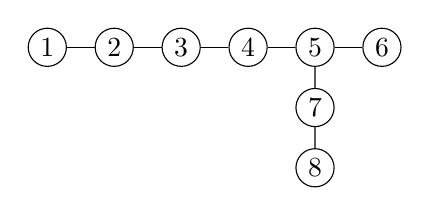
\begin{tikzpicture}[scale=.85,every node/.style={circle,draw,inner sep=2pt},every label/.style={font=\small}]
\foreach \i in {1,...,6}{\node (r\i) at (\i,0) {$\i$};}
\foreach \i [evaluate=\i as \j using int(\i+1)] in {1,...,5}{\draw (r\i)--(r\j);}
\node (r7) at (5,-.9) {$7$};\node (r8) at (5,-1.8) {$8$};\draw (r5)--(r7)--(r8);
\end{tikzpicture}
\end{center}
图上的数字是本题 $\alpha_i$ 的下标，与5.3中不带编号的图同构。

整数坐标且总和为偶数时，$\sum_i x_i^2\equiv\sum_i x_i\equiv0\pmod2$。半整数坐标可写为 $x_i=z_i+\tfrac12$，其中 $\sum_i z_i$ 为偶数，因而
\[
 (x,x)=\sum_i(z_i^2+z_i)+2
\]
也是偶整数。$L$ 对加减封闭，所以由极化公式知 $(x,y)\in\Z$。非零向量的长度平方因此至少为二。

设 $\Phi=\{\alpha\in L:(\alpha,\alpha)=2\}$。它有限，包含上述一组基，故张成 $\R^8$；同一直线上的根只有 $\pm\alpha$。对任一根，反射
\[
 s_\alpha(x)=x-(x,\alpha)\alpha
\]
保持 $L$，因为内积为整数；它又保持长度，所以置换 $\Phi$。且 $2(\beta,\alpha)/(\alpha,\alpha)=(\beta,\alpha)\in\Z$，满足晶体根系条件。因此 $\Phi$ 是约化晶体根系。

还要核对所给基是简单根系。若一个根的整数展开同时有正、负系数，写成 $\beta=\beta_+-\beta_-$，其中两部分是互不重叠的基向量正整数和。不同基向量内积非正，所以 $(\beta_+,\beta_-)\le0$；两个非零格向量的平方长度又都至少为二，于是
\[
 (\beta,\beta)=(\beta_+,\beta_+)+(\beta_-,\beta_-)-2(\beta_+,\beta_-)\ge4,
\]
与根长二矛盾。因此每个根的系数全非负或全非正，所给基确是简单根系。其Cartan图为 $E_8$，故根系类型为 $E_8$。

\textbf{(c)} 在 $x_1=x_2$ 的子空间中，取
\[
 e_3-e_4,\ e_4-e_5,\ e_5-e_6,\ e_6-e_7,\ e_7-e_8,\ e_7+e_8,
 \ -\frac12\sum_{i=1}^8e_i.
\]
前六个是最后六个坐标上 $D_6$ 的基。若共同坐标为 $a$，减去 $-2a$ 倍的最后一个向量，前两坐标化为零，剩下六个坐标为整数且总和为偶数。因此所写七个向量是这一子格的整数基。其内积图的三臂长度为 $(3,1,2)$，即 $E_7$。

在 $x_1=x_2=x_3$ 的子空间中，同样取
\[
 e_4-e_5,\ e_5-e_6,\ e_6-e_7,\ e_7-e_8,\ e_7+e_8,
 \ -\frac12\sum_{i=1}^8e_i.
\]
前五个生成最后五个坐标上的 $D_5$。减去 $-2a$ 倍最后一个向量后，前三坐标为零，最后五个坐标为整数且总和为偶数；总和的变化为 $-8a$，总是偶整数。所写六个向量遂为整数基，内积图的三臂长度为 $(2,1,2)$，即 $E_6$。这些子格中的根也构成根系：根的反射保持相应相等坐标子空间，前述根系检查原样适用；上述正、负系数矛盾也同样证明所写子格基是简单根系。

\textbf{(d)} 在 $E_8$ 中，整数根必须恰有两个非零坐标，各为 $\pm1$，因此为 $\pm e_i\pm e_j$，共 $4\binom82=112$ 个。半整数根的每个坐标绝对值至少为 $1/2$；长度平方为二迫使所有坐标都为 $\pm1/2$。总和为偶整数等价于负号个数为偶数，因此有 $2^7=128$ 个，合计 $240$。

对 $E_7$ 条件 $x_1=x_2$，整数根或者全部支撑在最后六个坐标上，共 $4\binom62=60$ 个；或者为 $\pm(e_1+e_2)$，另有两个。半整数根的前两符号相同；它们有两种选法，最后六个符号必须有偶数个负号，各有 $2^5$ 种。因此根数为
\[
 60+2+2\cdot2^5=126.
\]
对 $E_6$ 条件 $x_1=x_2=x_3$，整数根只能支撑在最后五个坐标上，共 $4\binom52=40$ 个。半整数根的前三符号全正时，后五个负号数须偶；前三全负时，后五个负号数须奇。两种情形各有 $2^4$ 种，故根数为
\[
 40+2\cdot2^4=72.
\]
两个计数都包含正根和负根，不能再乘二。
\end{solution}

\begin{exercise}\label{hw:5.41}
\textbf{MIT 18.712（2010）Homework 11 原题5.41；旧PDF第97页。}
设 $Q$ 为Dynkin箭图，$V_\alpha$ 是对应正根 $\alpha$ 的不可分解表示。简单根 $\alpha_i$ 对应的表示 $S_i=V_{\alpha_i}$ 只在顶点 $i$ 放置一维空间，其余顶点空间为零。
\begin{enumerate}[label=(\alph*)]
\item 若 $i$ 为源点（没有箭头进入），证明对任意表示 $V$，有 $\operatorname{Ext}^1(V,S_i)=0$；若 $i$ 为汇点（没有箭头离开），证明 $\operatorname{Ext}^1(S_i,V)=0$。
\item 对给定的箭头定向，构造 $V_\alpha$ 的Jordan--H\"older组成列。
\end{enumerate}
\end{exercise}
\begin{solution}
$\operatorname{Ext}^1(U,W)$ 的元素是短正合列 $0\to W\to E\to U\to0$ 的扩张类；它等于零表示所有这种列都能在表示范畴中分裂，而不只是向量空间能够分裂。

\textbf{(a)} 若 $i$ 是源点，考虑 $0\to S_i\to E\to V\to0$。除 $i$ 外，$E_j=V_j$；在 $i$ 取任一向量空间补空间 $L_i$，使 $E_i=(S_i)_i\oplus L_i$。从 $i$ 发出的所有箭头都在 $(S_i)_i$ 上为零，因为 $S_i$ 是子表示；从其他顶点进入 $i$ 的箭头则不存在。于是 $L_i$ 与其余全部 $E_j$ 一起构成一个子表示，与 $S_i$ 互补，故扩张分裂。

若 $i$ 是汇点，考虑 $0\to V\to E\to S_i\to0$。除 $i$ 外仍有 $E_j=V_j$，在 $i$ 取 $V_i$ 的一维补空间。由于没有离开 $i$ 的箭头，只在 $i$ 放置这个补空间就构成子表示，并同构于 $S_i$。所以扩张也分裂。这分别说明源点简单表示是内射对象、汇点简单表示是投射对象；本题并不需要一般投射覆盖或内射包理论。

\textbf{(b)} 底图是树，任意定向都无有向圈。先取一个汇点 $i_1$，删去它，再取剩余箭图的汇点 $i_2$，如此得到顺序 $i_1,\ldots,i_N$。等价地，每条箭头都从这个顺序中较后的顶点指向较前的顶点。

写 $\alpha=\sum_i n_i\alpha_i$，题设中的根对应意味着 $\dim(V_\alpha)_i=n_i$。定义 $U_r\subset V_\alpha$，使它在已选顶点 $i_1,\ldots,i_r$ 上等于全部顶点空间，在其余顶点为零。已选顶点不会向未选顶点发出箭头，因此各 $U_r$ 都是子表示，并有
\[
 0=U_0\subset U_1\subset\cdots\subset U_N=V_\alpha,
 \qquad U_r/U_{r-1}\cong S_{i_r}^{\oplus n_{i_r}}.
\]
在每个 $(V_\alpha)_{i_r}$ 中取任意完整旗标
$0\subset L_1\subset\cdots\subset L_{n_{i_r}}=(V_\alpha)_{i_r}$，用它把 $U_{r-1}\subset U_r$ 细分。细分时，流向更早顶点的箭头落在已经完整加入的空间中，进入当前顶点的未选空间为零，所以每一步仍为子表示。相邻商依次为
\[
 \underbrace{S_{i_1},\ldots,S_{i_1}}_{n_{i_1}\text{个}},\quad
 \underbrace{S_{i_2},\ldots,S_{i_2}}_{n_{i_2}\text{个}},\quad\ldots,\quad
 \underbrace{S_{i_N},\ldots,S_{i_N}}_{n_{i_N}\text{个}}.
\]
零重数的段略去。这就是对该定向的一条组成列，长度为 $\sum_i n_i$。该构造适用于任意无圈箭图表示，不依赖 $V_\alpha$ 不可分解；不可分解性也不意味着组成列只有一个商项。
\end{solution}
